\documentclass{article}
%--PASTE INTO MAIN FILE--
% \documentclass{article}
% %--PASTE INTO MAIN FILE--
% \documentclass{article}
% %--PASTE INTO MAIN FILE--
% \documentclass{article}
% \input{TexBase/DocumentBase.tex}
% \end{document}

\usepackage[margin = 0.7in]{geometry}
\usepackage{graphicx}
\usepackage{graphics}
\usepackage[T1]{fontenc}
\usepackage[polish]{babel}
\usepackage{cmap}
\usepackage[utf8]{inputenc}
\usepackage{float}
\usepackage{tabularx}
\usepackage[table,xcdraw]{xcolor}
\usepackage{lipsum}
\usepackage{titlesec}
\usepackage{minted}
\usepackage{xcolor}
\usepackage{caption}
\usepackage{enumitem}
\usepackage{csvsimple}
\usepackage{natbib}
\usepackage{blindtext}

\usepackage{amsmath} %math

\usepackage{numprint} % rounding
\usepackage[round-precision=3,round-mode=figures, scientific-notation=true]{siunitx} %scientific notation

\usepackage[hidelinks]{hyperref}
\usepackage{url}

\usepackage{bm} %bold for math


%TABS
\usepackage[]{booktabs}
\usepackage{tabularray}
\usepackage{multirow}

%\title{}
\author{Michał Dziedziak}
\date{\today}


\titlespacing\section{0pt}{12pt plus 4pt minus 2pt}{0pt plus 2pt minus 2pt}
\titlespacing\subsection{0pt}{12pt plus 4pt minus 2pt}{0pt plus 2pt minus 2pt}
\titlespacing\subsubsection{0pt}{12pt plus 4pt minus 2pt}{0pt plus 2pt minus 2pt}
\setlength{\parskip}{\baselineskip}%
\setlength{\parindent}{0pt}%

\newcommand{\squeezeup}{\vspace{-5mm}}


\begin{document}

\begin{titlepage}
    \begin{center}
        \vspace*{5cm}
        \rule{500pt}{1pt}\\
        \vspace*{0.5cm}
        \LARGE
        \textbf{Inżyniera Obrazów}\\
        \Large
        Laboratorium numer 2
        \vspace*{0.5cm}
        \rule{500pt}{1pt}
    \end{center}

    \vspace*{10cm}

    {\raggedright
        \large
        \textbf{Autor sprawozdania:} Michał Dziedziak 263901\\
        \textbf{Imię i Nazwisko prowadzącego kurs:} dr inż. Jan Nikodem\\
        \textbf{Dzień i godzina zajęć:} czwartek, 11:15 - 14:15
    }
\end{titlepage}


\tableofcontents
% \listoftables

%\renewcommand\listoflistingscaption{List of source codes}
% \listoflistings

\listoffigures


\newpage


% \begin{table}[H]
%     \centering
%     \begin{tabular}{|c|c|c|c|}%
%         \hline
%         \bfseries Numer iteracji & \bfseries Czas zalezienia rozwiązania [ms] & Koszt ścieżki & Błąd względny% specify table head
%         \csvreader[head to column names]{Csv/BestPathTest_SimulatedAnnealing_LINEAR_ftv47.csv}{}% use head of csv as column names
%         {\\\hline\Iteration & \num{\TimeInMiliSeconds} & \Cost & \num[round-precision=2, round-mode=places, scientific-notation=false]{\Error}\%}% specify your columns here
%         \\\hline    
%     \end{tabular}
%     \caption{}
%     \label{tab:}
% \end{table}

% \begin{figure}[H]
%     \centering
%     \resizebox{\columnwidth}{!}{%
%     \includegraphics{}%
%     }
%     \caption{}
%     \label{fig:}
% \end{figure}

% \begin{listing}[H]
%     \begin{minted}[frame=single,framesep=2mm,linenos,fontsize=\footnotesize]{language}
%         some code
%     \end{minted}
%     \caption{}
%     \label{lst:}
% \end{listing}


% \bibliographystyle{plainnat}
% \bibliography{TexBase/Bibliography}

% \end{document}

\usepackage[margin = 0.7in]{geometry}
\usepackage{graphicx}
\usepackage{graphics}
\usepackage[T1]{fontenc}
\usepackage[polish]{babel}
\usepackage{cmap}
\usepackage[utf8]{inputenc}
\usepackage{float}
\usepackage{tabularx}
\usepackage[table,xcdraw]{xcolor}
\usepackage{lipsum}
\usepackage{titlesec}
\usepackage{minted}
\usepackage{xcolor}
\usepackage{caption}
\usepackage{enumitem}
\usepackage{csvsimple}
\usepackage{natbib}
\usepackage{blindtext}

\usepackage{amsmath} %math

\usepackage{numprint} % rounding
\usepackage[round-precision=3,round-mode=figures, scientific-notation=true]{siunitx} %scientific notation

\usepackage[hidelinks]{hyperref}
\usepackage{url}

\usepackage{bm} %bold for math


%TABS
\usepackage[]{booktabs}
\usepackage{tabularray}
\usepackage{multirow}

%\title{}
\author{Michał Dziedziak}
\date{\today}


\titlespacing\section{0pt}{12pt plus 4pt minus 2pt}{0pt plus 2pt minus 2pt}
\titlespacing\subsection{0pt}{12pt plus 4pt minus 2pt}{0pt plus 2pt minus 2pt}
\titlespacing\subsubsection{0pt}{12pt plus 4pt minus 2pt}{0pt plus 2pt minus 2pt}
\setlength{\parskip}{\baselineskip}%
\setlength{\parindent}{0pt}%

\newcommand{\squeezeup}{\vspace{-5mm}}


\begin{document}

\begin{titlepage}
    \begin{center}
        \vspace*{5cm}
        \rule{500pt}{1pt}\\
        \vspace*{0.5cm}
        \LARGE
        \textbf{Inżyniera Obrazów}\\
        \Large
        Laboratorium numer 2
        \vspace*{0.5cm}
        \rule{500pt}{1pt}
    \end{center}

    \vspace*{10cm}

    {\raggedright
        \large
        \textbf{Autor sprawozdania:} Michał Dziedziak 263901\\
        \textbf{Imię i Nazwisko prowadzącego kurs:} dr inż. Jan Nikodem\\
        \textbf{Dzień i godzina zajęć:} czwartek, 11:15 - 14:15
    }
\end{titlepage}


\tableofcontents
% \listoftables

%\renewcommand\listoflistingscaption{List of source codes}
% \listoflistings

\listoffigures


\newpage


% \begin{table}[H]
%     \centering
%     \begin{tabular}{|c|c|c|c|}%
%         \hline
%         \bfseries Numer iteracji & \bfseries Czas zalezienia rozwiązania [ms] & Koszt ścieżki & Błąd względny% specify table head
%         \csvreader[head to column names]{Csv/BestPathTest_SimulatedAnnealing_LINEAR_ftv47.csv}{}% use head of csv as column names
%         {\\\hline\Iteration & \num{\TimeInMiliSeconds} & \Cost & \num[round-precision=2, round-mode=places, scientific-notation=false]{\Error}\%}% specify your columns here
%         \\\hline    
%     \end{tabular}
%     \caption{}
%     \label{tab:}
% \end{table}

% \begin{figure}[H]
%     \centering
%     \resizebox{\columnwidth}{!}{%
%     \includegraphics{}%
%     }
%     \caption{}
%     \label{fig:}
% \end{figure}

% \begin{listing}[H]
%     \begin{minted}[frame=single,framesep=2mm,linenos,fontsize=\footnotesize]{language}
%         some code
%     \end{minted}
%     \caption{}
%     \label{lst:}
% \end{listing}


% \bibliographystyle{plainnat}
% \bibliography{TexBase/Bibliography}

% \end{document}

\usepackage[margin = 0.7in]{geometry}
\usepackage{graphicx}
\usepackage{graphics}
\usepackage[T1]{fontenc}
\usepackage[polish]{babel}
\usepackage{cmap}
\usepackage[utf8]{inputenc}
\usepackage{float}
\usepackage{tabularx}
\usepackage[table,xcdraw]{xcolor}
\usepackage{lipsum}
\usepackage{titlesec}
\usepackage{minted}
\usepackage{xcolor}
\usepackage{caption}
\usepackage{enumitem}
\usepackage{csvsimple}
\usepackage{natbib}
\usepackage{blindtext}

\usepackage{amsmath} %math

\usepackage{numprint} % rounding
\usepackage[round-precision=3,round-mode=figures, scientific-notation=true]{siunitx} %scientific notation

\usepackage[hidelinks]{hyperref}
\usepackage{url}

\usepackage{bm} %bold for math


%TABS
\usepackage[]{booktabs}
\usepackage{tabularray}
\usepackage{multirow}

%\title{}
\author{Michał Dziedziak}
\date{\today}


\titlespacing\section{0pt}{12pt plus 4pt minus 2pt}{0pt plus 2pt minus 2pt}
\titlespacing\subsection{0pt}{12pt plus 4pt minus 2pt}{0pt plus 2pt minus 2pt}
\titlespacing\subsubsection{0pt}{12pt plus 4pt minus 2pt}{0pt plus 2pt minus 2pt}
\setlength{\parskip}{\baselineskip}%
\setlength{\parindent}{0pt}%

\newcommand{\squeezeup}{\vspace{-5mm}}


\begin{document}

\begin{titlepage}
    \begin{center}
        \vspace*{5cm}
        \rule{500pt}{1pt}\\
        \vspace*{0.5cm}
        \LARGE
        \textbf{Inżyniera Obrazów}\\
        \Large
        Laboratorium numer 2
        \vspace*{0.5cm}
        \rule{500pt}{1pt}
    \end{center}

    \vspace*{10cm}

    {\raggedright
        \large
        \textbf{Autor sprawozdania:} Michał Dziedziak 263901\\
        \textbf{Imię i Nazwisko prowadzącego kurs:} dr inż. Jan Nikodem\\
        \textbf{Dzień i godzina zajęć:} czwartek, 11:15 - 14:15
    }
\end{titlepage}


\tableofcontents
% \listoftables

%\renewcommand\listoflistingscaption{List of source codes}
% \listoflistings

\listoffigures


\newpage


% \begin{table}[H]
%     \centering
%     \begin{tabular}{|c|c|c|c|}%
%         \hline
%         \bfseries Numer iteracji & \bfseries Czas zalezienia rozwiązania [ms] & Koszt ścieżki & Błąd względny% specify table head
%         \csvreader[head to column names]{Csv/BestPathTest_SimulatedAnnealing_LINEAR_ftv47.csv}{}% use head of csv as column names
%         {\\\hline\Iteration & \num{\TimeInMiliSeconds} & \Cost & \num[round-precision=2, round-mode=places, scientific-notation=false]{\Error}\%}% specify your columns here
%         \\\hline    
%     \end{tabular}
%     \caption{}
%     \label{tab:}
% \end{table}

% \begin{figure}[H]
%     \centering
%     \resizebox{\columnwidth}{!}{%
%     \includegraphics{}%
%     }
%     \caption{}
%     \label{fig:}
% \end{figure}

% \begin{listing}[H]
%     \begin{minted}[frame=single,framesep=2mm,linenos,fontsize=\footnotesize]{language}
%         some code
%     \end{minted}
%     \caption{}
%     \label{lst:}
% \end{listing}


% \bibliographystyle{plainnat}
% \bibliography{TexBase/Bibliography}


\section{Temat laboratorium}
Steganografia jest dziedziną nauki zajmującą się ukrywaniem komunikatów w jawnym medium.
W ramach tego laboratorium, eksplorujemy techniki steganograficzne,
koncentrując się na metodzie ukrywania informacji w obrazach poprzez modyfikację ich najmniej znaczących bitów (LSB - Least Significant Bit).

W praktyce używamy metody, która zapisuję ukrytą informację w obrazie poprzez modyfikację n-wybranych
ostatnich bitów pikseli obrazu.

\section{Zadanie 1}
\subsection{Treść}
Pierwsze zadanie polegało o użyciu gotowych funkcji \textit{hide\_message} oraz \textit{reveal\_message} w
celu zakodowania i odkodowania wiadomości w obrazie.

Zadanie zostało rozbudowane o menu, umożliwiające wybór czynności: \textit{zakodowanie wiadomości},
\textit{odkodowanie wiadomości}.
Pozwala ono na zapisania obrazu z zakodowaną wiadomością do pliku, oraz odczytanie wiadomości z obrazu z
pliku, który może pochodzić z innego programu.

\subsection{Prezentacja wykonanego zadania}

\subsubsection*{Kodowanie wiadomości}
\begin{figure}[H]
    \centering
    \resizebox{\columnwidth}{!}{%
        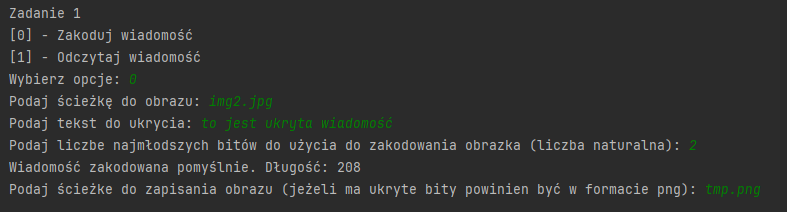
\includegraphics{img/zad1_2.png}%
    }
    \caption{Zdjęcie konsoli podczas kodowania wiadomości}
\end{figure}

\begin{figure}[H]
    \centering
    \resizebox{\columnwidth}{!}{%
        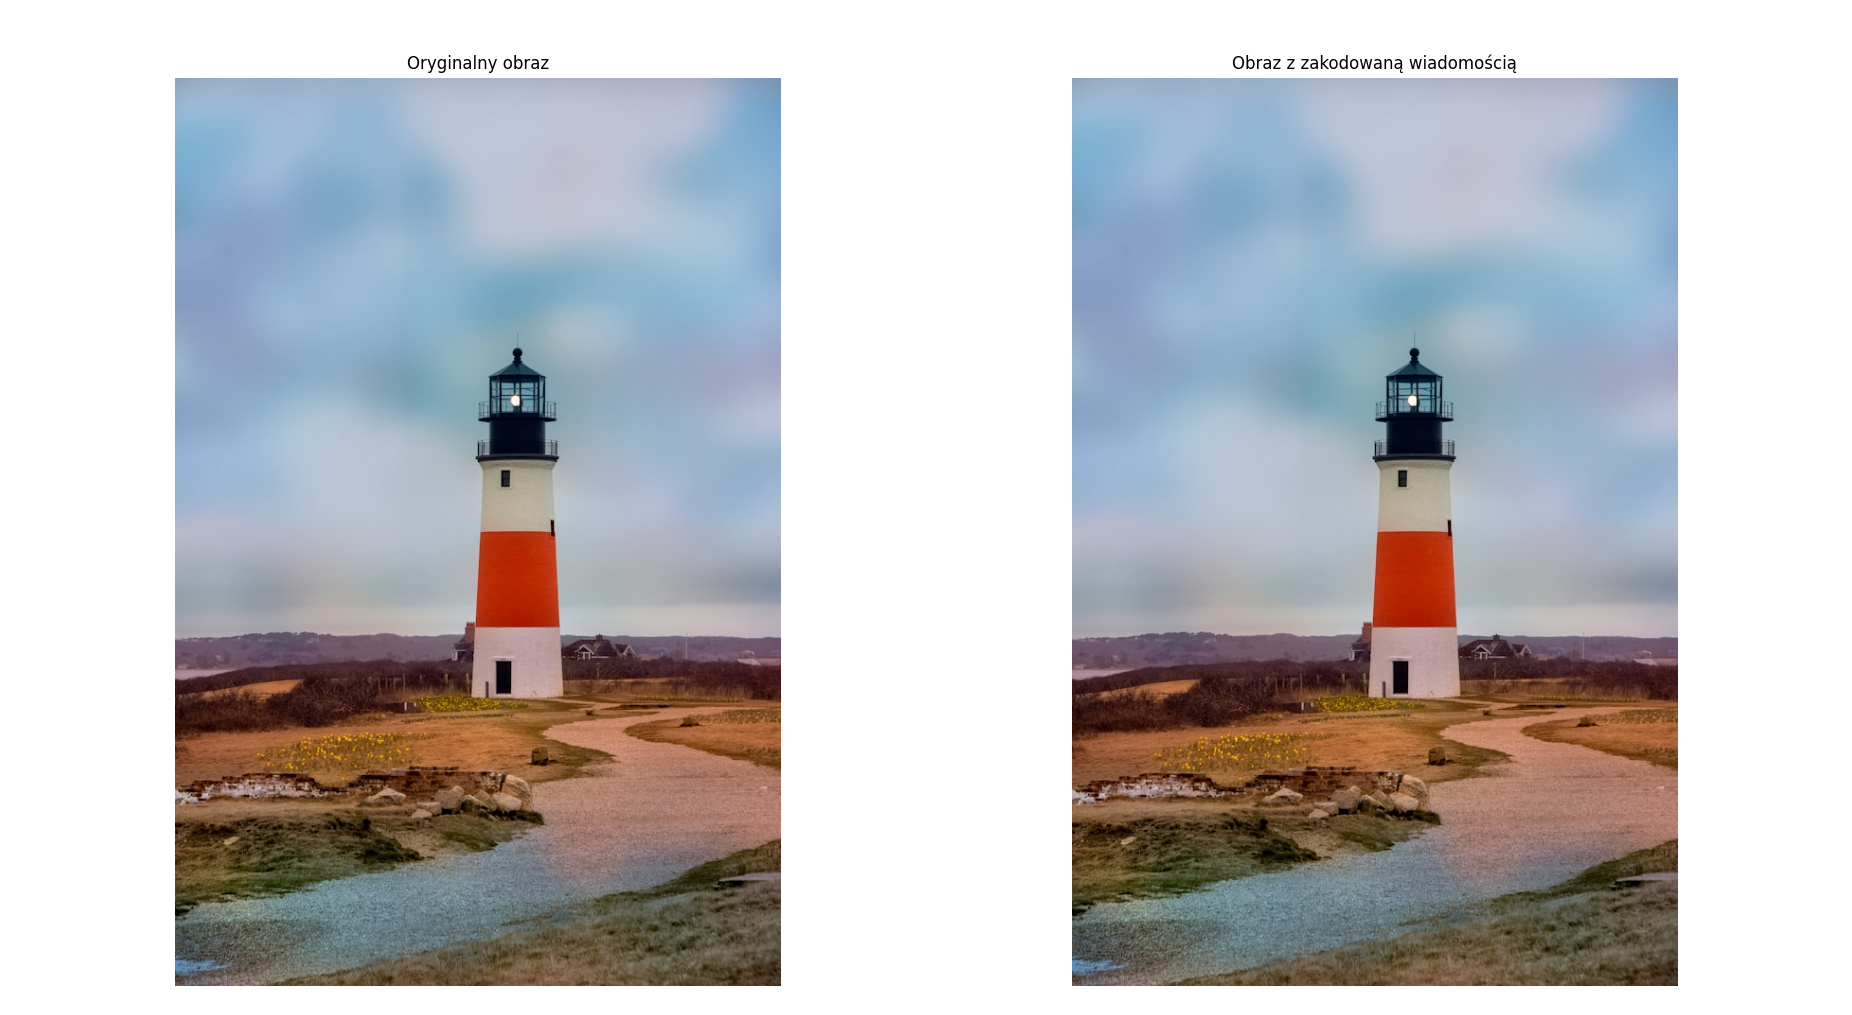
\includegraphics{img/zad1.png}%
    }
    \caption{Zdjęcie z zakodowaną wiadomością}
\end{figure}

\subsubsection*{Dekodowanie wiadomości}
\begin{figure}[H]
    \centering
    \resizebox{\columnwidth}{!}{%
        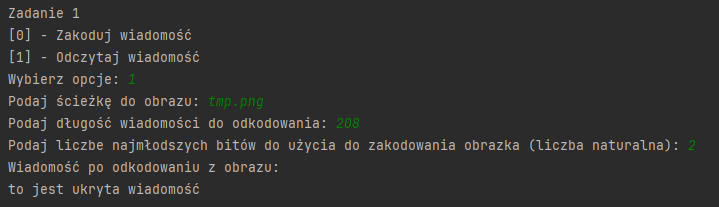
\includegraphics{img/zad1_3.png}%
    }
    \caption{Zdjęcie konsoli podczas dekodowania wiadomości}
\end{figure}



\section{Zadanie 2}
\subsection{Treść}
W zadaniu drugim nalezało zakodować w obrazie wiadomość o długości 75\% liczby bajtów w obrazie.
Następnie należało zmierzyć wartości MSE pomiędzy oryginalnym obrazem o obrazem z zakodowaną wiadomością
dla wartości \textit{nbits} od 1 do 8.

\subsection{Prezentacja wykonanego zadania}
\begin{figure}[H]
    \centering
    \resizebox{\columnwidth}{!}{%
        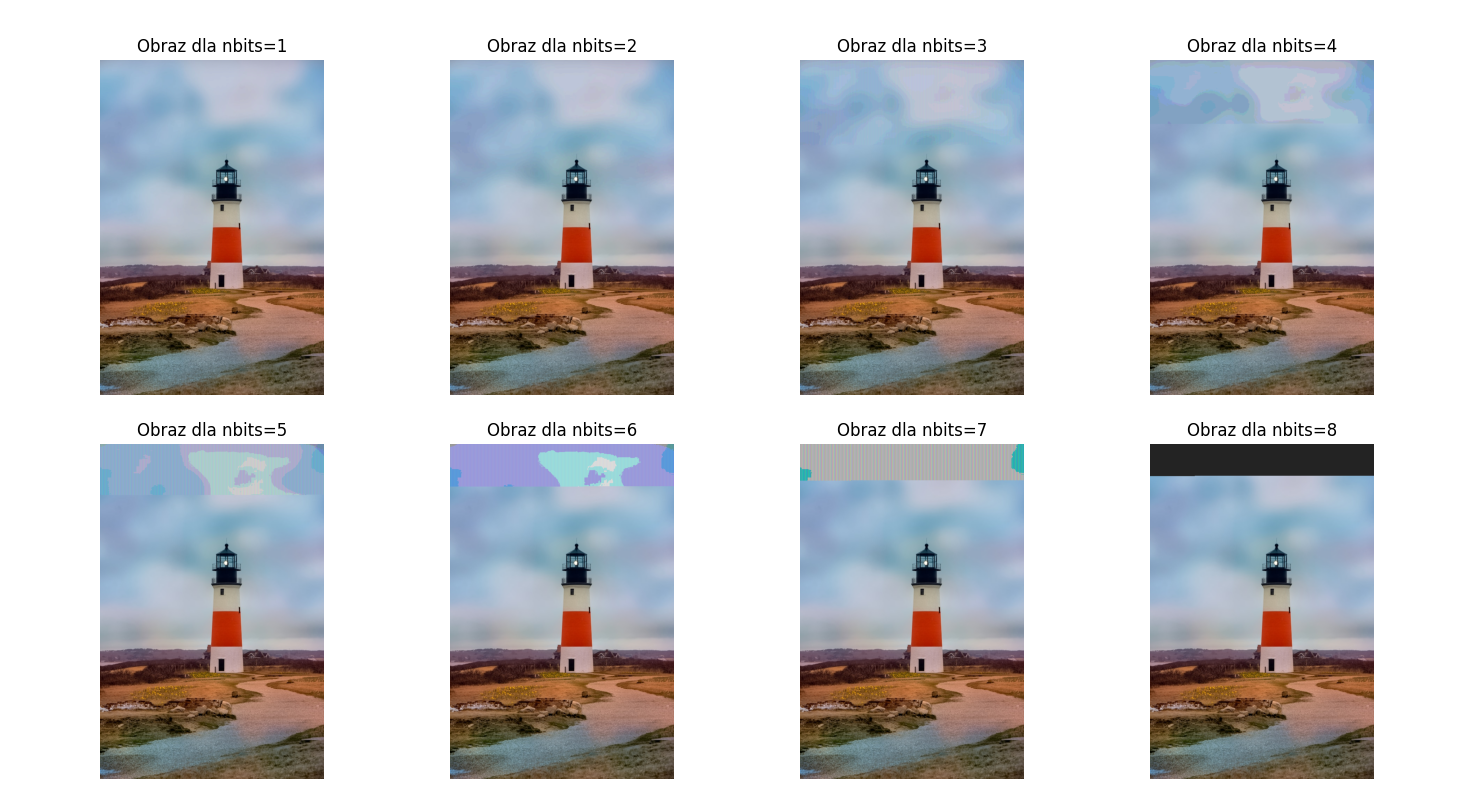
\includegraphics{img/zad2.png}%
    }
    \caption{Obrazy z kolejnymi wartościami nbits}
\end{figure}

\begin{figure}[H]
    \centering
    \resizebox{\columnwidth}{!}{%
        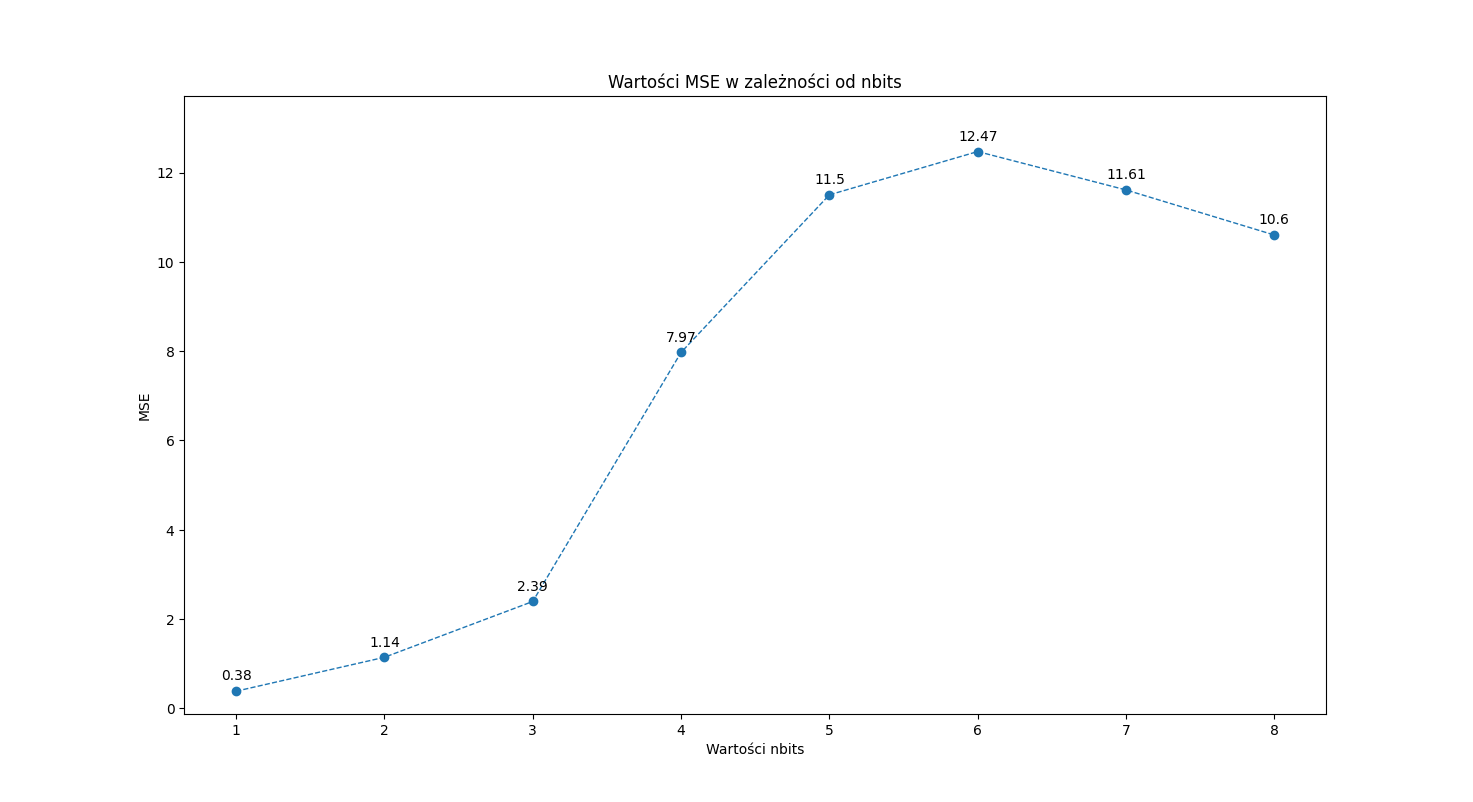
\includegraphics{img/zad2_plot.png}%
    }
    \caption{Wykres zależności MSE od wartości nbits}
\end{figure}

% TODO wnioski?


\section{Zadanie 3}
\subsection{Treść}
W zadaniu trzecim należało zmodyfikować funkcję \textit{hide\_message} i \textit{reveal\_message} tak,
aby można było wybrać od którego miejsca ma być zapisywana wiadomość w obrazie.

Zadanie zostało rozbudowane o menu analogiczne do tego z zadania pierwszego.

% TODO jakoś opisać jak to zrobiłem
\subsection{Prezentacja wykonanego zadania}

\subsubsection*{Kodowanie wiadomości}
\begin{figure}[H]
    \centering
    \resizebox{\columnwidth}{!}{%
        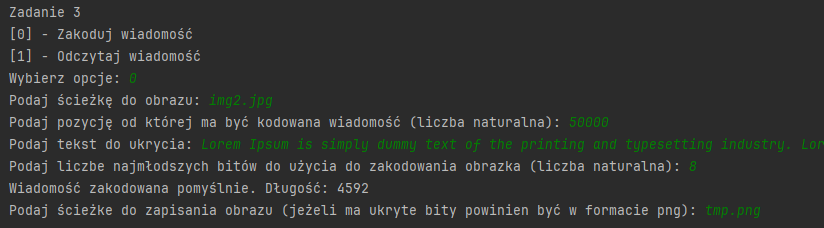
\includegraphics{img/zad3_2.png}%
    }
    \caption{Zdjęcie logów konsoli podczas procesu kodowania wiadomości}
\end{figure}

\begin{figure}[H]
    \centering
    \resizebox{\columnwidth}{!}{%
        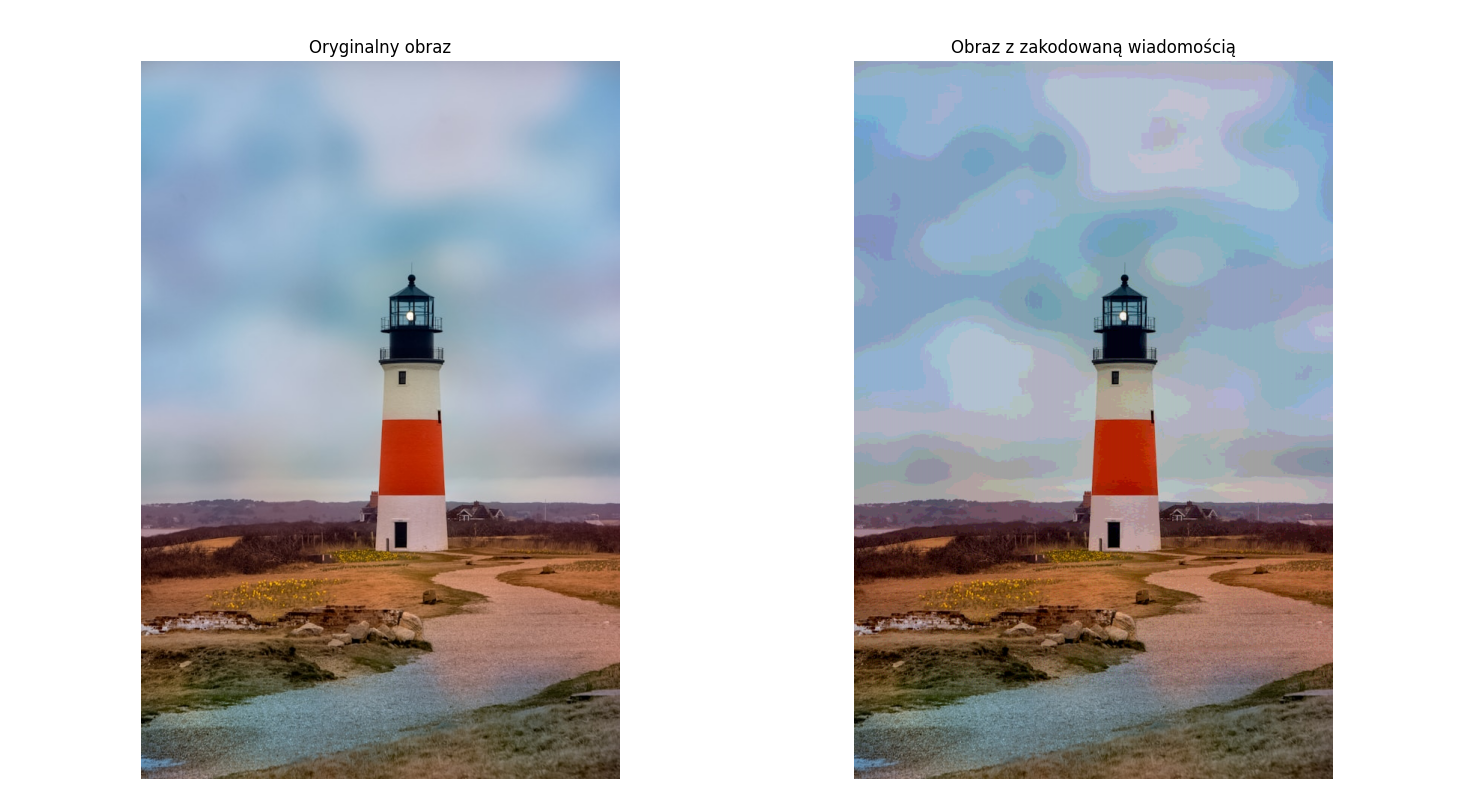
\includegraphics{img/zad3.png}%
    }
    \caption{Obraz przed i po zakodowaniu wiadomości od pozycji 50000}
\end{figure}


\subsubsection*{Dekodowanie wiadomości}
\begin{figure}[H]
    \centering
    \resizebox{\columnwidth}{!}{%
        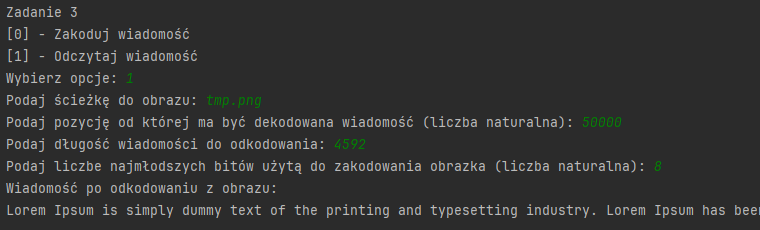
\includegraphics{img/zad3_3.png}%
    }
    \caption{Zdjęcie logów konsoli podczas procesu dekodowania wiadomości}
\end{figure}


\section{Zadanie 4}
\subsection{Treść}
Zadanie czwarte polegało na zaimplementowaniu funkcjonalności ukrywania (i odzyskiwania) obrazu w innym
obrazie.

W praktyce oznaczało to dodanie kroku, który spłaszczał piksele w obrazie do jednego wymiaru, a następnie
ukrywał kolejne bity w najmniej znaczących bitach obrazu docelowego.

Analogicznie proces odzyskiwania obrazu polegał na odczytaniu ukrytych bitów i odpowiednią ich transformację
do kanałów RGB.

Zadanie zostało rozbudowane o menu analogiczne do tego z zadania pierwszego.

\subsection{Prezentacja wykonanego zadania}

\subsubsection*{Kodowanie obrazu}
\begin{figure}[H]
    \centering
    \resizebox{\columnwidth}{!}{%
        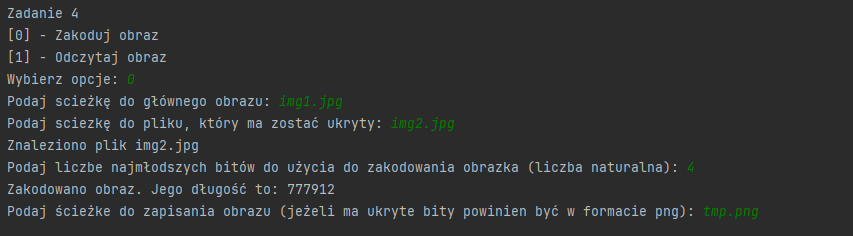
\includegraphics{img/zad4_2.png}%
    }
    \caption{Zdjęcie logów konsoli podczas procesu ukrywania obrazu w innym obrazie}
\end{figure}

\begin{figure}[H]
    \centering
    \resizebox{\columnwidth}{!}{%
        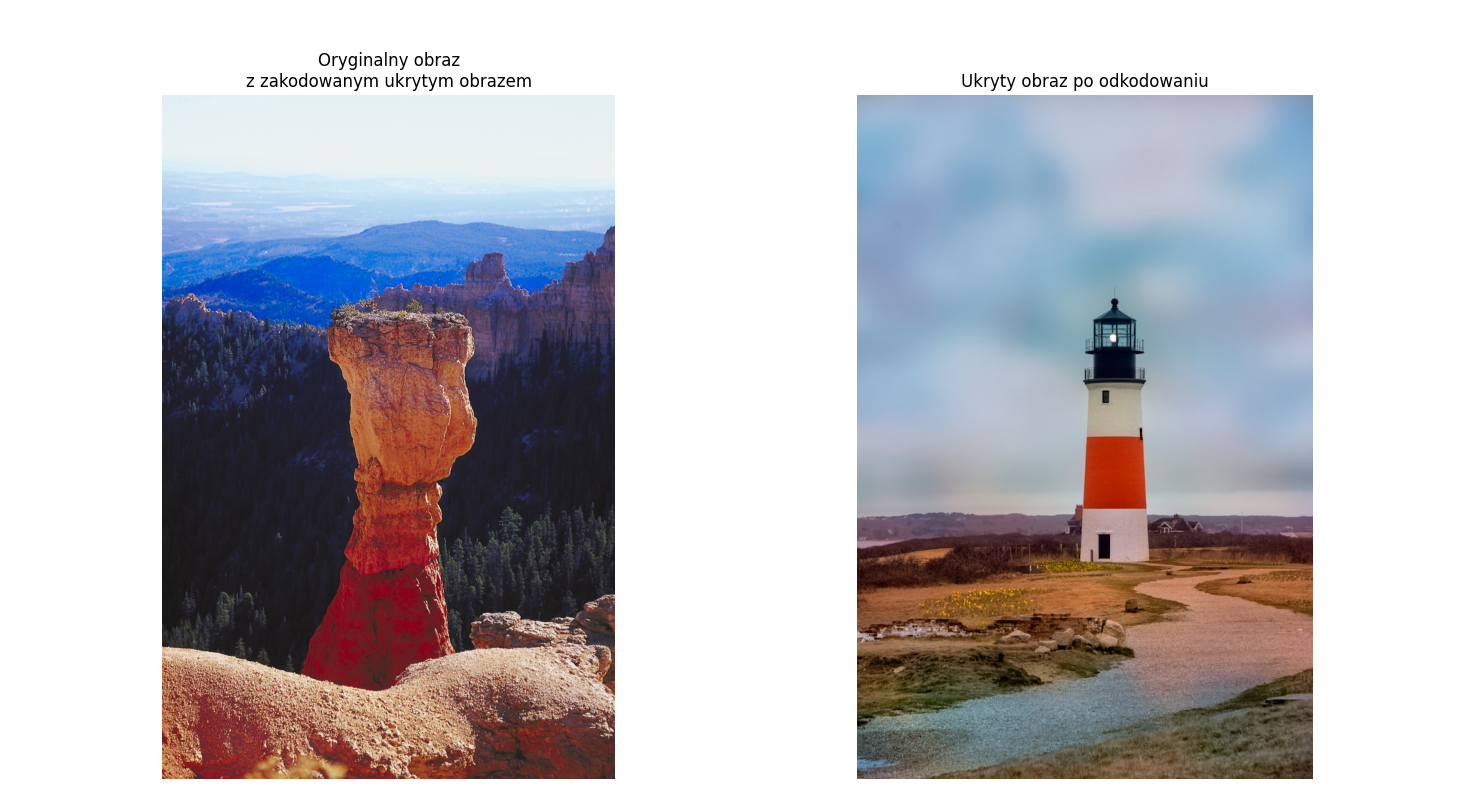
\includegraphics{img/zad4.png}%
    }
    \caption{Prezentacja obrazu przed i po zakodowaniu w nim innego obrazu}
\end{figure}

\subsubsection*{Dekodowanie obrazu}
\begin{figure}[H]
    \centering
    \resizebox{\columnwidth}{!}{%
        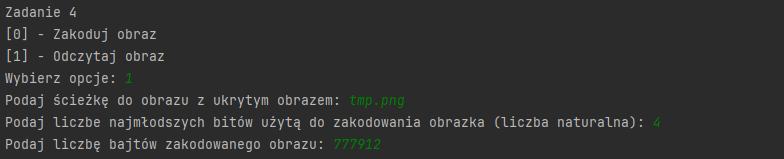
\includegraphics{img/zad4_4.png}%
    }
    \caption{Zdjęcie logów konsoli podczas procesu odzyskiwania obrazu z innego obrazu}
\end{figure}

\begin{figure}[H]
    \centering
    \resizebox{\columnwidth}{!}{%
        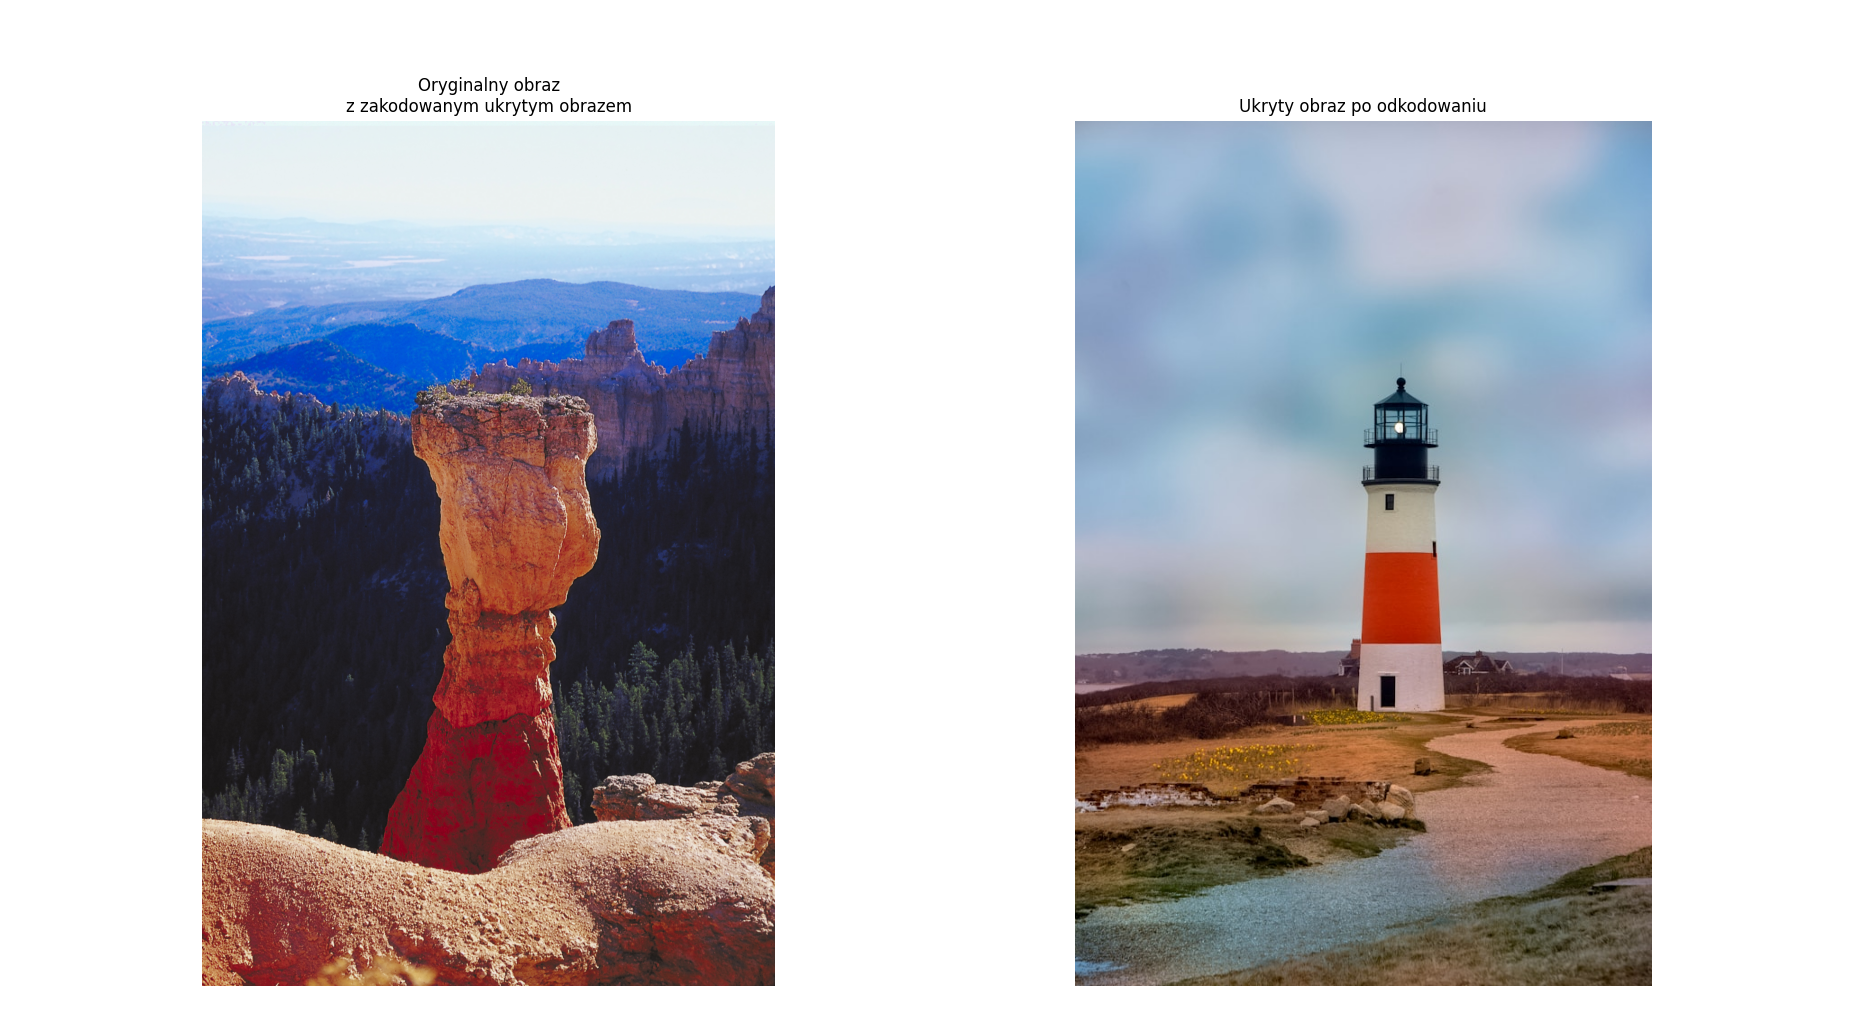
\includegraphics{img/zad4_3.png}%
    }
    \caption{Prezentacja obrazu z ukrytym obrazem oraz odkodowanego obrazu}
\end{figure}

\section{Zadanie 5}
\subsection{Treść}
W zadaniu piątym należało rozbudować odczytywanie obrazu z pliku o automatyczne wykrywanie końca wiadomości.
W ramach zadania zaimplementowałem rozpoznawanie końca wiadomości poprzez sprawdzanie czy aktualnie
przetwarzane bajty pokrywają się ze stopką konca pliku jpg:
\[\text{kod stopki} =1111 1111 1101 1001_2 = FFD9_{16}\]

\subsection{Prezentacja wykonanego zadania}
\begin{figure}[H]
    \centering
    \resizebox{\columnwidth}{!}{%
        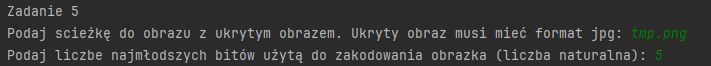
\includegraphics{img/zad5_2.png}%
    }
    \caption{Zdjęcie logów konsoli podczas procesu odzyskiwania obrazu z innego obrazu}
\end{figure}

\begin{figure}[H]
    \centering
    \resizebox{\columnwidth}{!}{%
        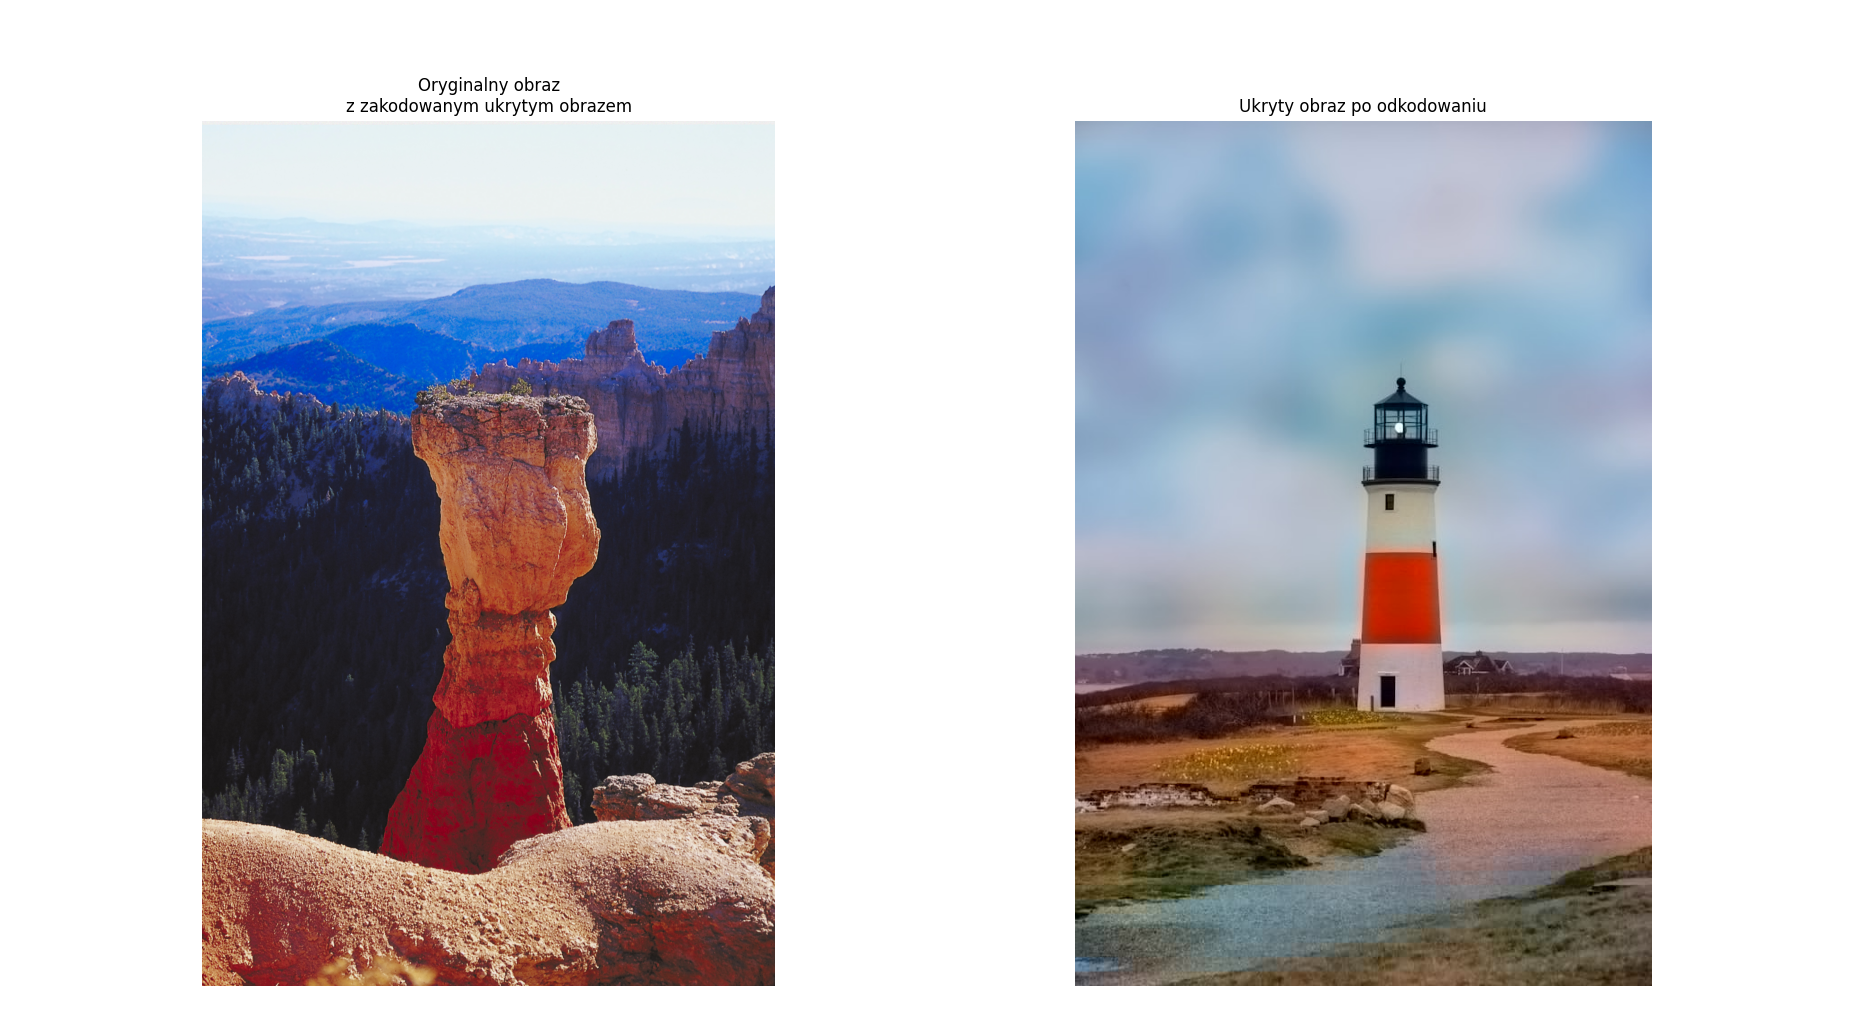
\includegraphics{img/zad5.png}%
    }
    \caption{Prezentacja obrazu z ukrytym obrazem oraz odkodowanego obrazu}
\end{figure}

\end{document}